% *** ก่อนส่ง: ลบข้อความตัวอย่าง (\ldots) ทั้งหมด แล้วเขียนเนื้อหาของตนเอง ***
% =============================================================
% บทที่ 3 - วิธีการดำเนินงาน
% แก้ไขเนื้อหาในบทนี้ได้ที่ไฟล์ chapter3.tex
% =============================================================

% อธิบายขั้นตอนและวิธีการดำเนินงาน
% รวมถึงเครื่องมือที่ใช้ในการทำโครงงาน

% -----------------------------------------------------------
\section{ขั้นตอนการดำเนินงาน}
% -----------------------------------------------------------

โครงงานนี้ดำเนินงานตามขั้นตอน ดังนี้

\subsection{ศึกษาและวิเคราะห์ความต้องการ}

ขั้นตอนนี้เป็นพื้นฐานในการกำหนดขอบเขตและเทคโนโลยีที่จำเป็นต่อการพัฒนา

\subsubsection{การศึกษาทฤษฎีและงานวิจัยที่เกี่ยวข้อง}

\paragraph{ทบทวนหลักการของระบบแนะนำ}
ศึกษาพื้นฐานของ Collaborative Filtering และ Deep Learning

\paragraph{เทคนิค Multi-Behavior Learning}
ศึกษาหลักการของโมเดล MB-CGCN (Multi-Behavior Recommendation with Cascading Graph Convolution Networks) ซึ่งมีความโดดเด่นในการจัดการข้อมูลพฤติกรรมที่มีความต่อเนื่องเป็นลำดับขั้น เช่น เริ่มจากการคลิกอ่านเนื้อหา ไปสู่การเพิ่มลงในตะกร้า และจบที่การเช่า ซึ่งเป็นพฤติกรรมเป้าหมาย โดยโมเดลนี้จะใช้เทคนิค Cascading GCN ผสานกับ Feature Transformation ในการส่งต่อและคัดกรองฟีเจอร์สำคัญจากพฤติกรรมก่อนหน้า เพื่อนำไปช่วยเพิ่มความแม่นยำในการทำนายพฤติกรรมเป้าหมายได้อย่างมีประสิทธิภาพ \cite{mbcgcn_nd}

\paragraph{สถาปัตยกรรม Deep Learning}
การใช้ PyTorch ในการสร้าง Graph Neural Networks

\paragraph{เมทริกซ์การประเมินผล}
ศึกษาตัวชี้วัด Ranking Metrics เช่น NDCG และ Recall

\subsubsection{การวิเคราะห์พฤติกรรมผู้ใช้}

\paragraph{การกำหนดและนิยามข้อมูลพฤติกรรมผู้ใช้}
พฤติกรรมของผู้ใช้ในระบบแนะนำหนังสือการ์ตูนสำหรับการเช่าอ่าน สามารถแบ่งออกเป็น 3 ประเภท ได้แก่ พฤติกรรมการคลิกอ่านเนื้อหา พฤติกรรมตะกร้า และพฤติกรรมการเช่า เพื่อใช้ในการฝึกฝนโมเดล

\paragraph{พฤติกรรมการคลิกอ่านเนื้อหา}
คือการที่ผู้ใช้เปิดหน้ารายละเอียดของหนังสือการ์ตูน พฤติกรรมนี้เป็นสัญญาณแรกสุดที่แสดงถึงความสนใจของผู้ใช้ก่อนการตัดสินใจเช่า ระบบบันทึกเป็นเหตุการณ์ click ในตาราง UserBehaviorLog ทุกครั้งที่หน้ารายละเอียดโหลดสำเร็จ และใช้เป็นข้อมูลเสริมให้กับโมเดลที่สอง

\paragraph{พฤติกรรมการกดเข้าตะกร้า}
คือการที่ผู้ใช้เพิ่มหนังสือลงในรายการที่ตั้งใจจะเช่า ในโมเดลที่หนึ่ง อ้างอิงจากสถานะ "Plan to Watch" ของชุดข้อมูล MyAnimeList ส่วนในเว็บแอปพลิเคชันบันทึกเป็นเหตุการณ์ ADD CART เมื่อการเพิ่มลงตะกร้าสำเร็จ พฤติกรรมนี้แสดงถึงความสนใจที่มากขึ้นและความตั้งใจที่จะเช่าในอนาคต

\paragraph{พฤติกรรมการเช่า}
คือการที่ผู้ใช้ยืนยันคำขอเช่าหนังสือการ์ตูน ในโมเดลที่หนึ่ง อ้างอิงจากสถานะ "Watching" และ "Completed" ของชุดข้อมูล MyAnimeList ส่วนในเว็บแอปพลิเคชัน เซิร์ฟเวอร์บันทึกเหตุการณ์ RENT อัตโนมัติสำหรับหนังสือทุกเล่มในตะกร้าเมื่อผู้ใช้กดยืนยันการจอง พฤติกรรมนี้เป็นตัวชี้วัดความชอบสูงสุดและเป็นพฤติกรรมเป้าหมายสุดท้ายในห่วงโซ่ที่ต้องการให้ระบบทำนายผล

\paragraph{การนำไปใช้ในโมเดล}

\paragraph{การเปรียบเทียบ}
สำหรับโมเดลพื้นฐาน จะถูกฝึกฝนโดยใช้ข้อมูลการเช่า เพียงอย่างเดียว

\paragraph{โมเดล MB-CGCN}
จะใช้วิธีการจัดเรียงพฤติกรรมให้เป็นห่วงโซ่ความสัมพันธ์ โดยพัฒนา 2 รุ่น ได้แก่ รุ่น v1 ใช้ห่วงโซ่ 2 ขั้น Cart $\rightarrow$ Rent ที่สร้างจากชุดข้อมูล MyAnimeList และรุ่น v2 ใช้ห่วงโซ่ 3 ขั้น View $\rightarrow$ Cart $\rightarrow$ Rent ที่สร้างจาก Log พฤติกรรมในตาราง UserBehaviorLog ของเว็บแอปพลิเคชัน กระบวนการทำงานของรุ่น v2 เริ่มจากการเรียนรู้ลักษณะของผู้ใช้จากพฤติกรรมการคลิกก่อน จากนั้นแปลงเวกเตอร์ด้วยเมทริกซ์แปลงค่าเพื่อคัดกรองสัญญาณรบกวน แล้วส่งต่อไปเป็นค่าเริ่มต้นของการเรียนรู้พฤติกรรมตะกร้า และส่งต่อไปยังพฤติกรรมการเช่าซึ่งเป็นพฤติกรรมเป้าหมายในลักษณะเดียวกัน รุ่น v1 ทำงานแบบเดียวกันแต่เริ่มที่พฤติกรรมตะกร้า เนื่องจากชุดข้อมูล MyAnimeList ไม่มีพฤติกรรมการคลิก ผลการทดสอบของทั้งสองรุ่นแสดงในบทที่ 4 ผลการทดลองเปรียบเทียบลำดับพฤติกรรมในช่วงศึกษาแนวคิดแสดงดังภาพที่ \ref{fig:graph}

\begin{figure}[H]
\centering
% \includegraphics[width=0.9\textwidth]{images/usecase.png}
{\centering\vspace{1cm}\textit{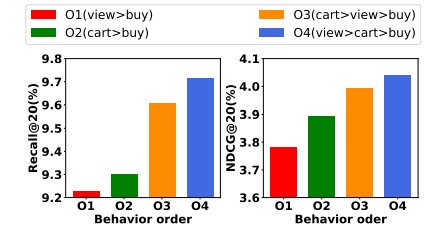
\includegraphics[width=0.9\textwidth]{images/3image8.png}}\vspace{1cm}}
\caption{กราฟแสดงผลการทดลองเปรียบเทียบลำดับพฤติกรรมที่แตกต่างกัน \cite{mltestscore_nd}}
\label{fig:graph}
\end{figure}

กราฟนี้แสดงผลการทดลองเปรียบเทียบลำดับพฤติกรรมที่แตกต่างกัน 2 รูปแบบ ได้แก่ Cart $\rightarrow$ Rent (Behavior 2) และ View $\rightarrow$ Cart $\rightarrow$ Rent (Behavior 3) โดยแกนนอนคือจำนวน Epoch ที่ฝึกสอน และแกนตั้งคือค่า Recall@20 ซึ่งวัดความแม่นยำของการจัดอันดับแนะนำ ตัวอย่างเช่น ถ้าโมเดลแนะนำหนังสือ 20 เล่มแรกแล้วมีหนังสือที่ผู้ใช้สนใจเช่าจริงอยู่ในนั้น 4 เล่ม ค่า Recall@20 จะเท่ากับ 0.20 จากกราฟจะเห็นว่าโมเดล Behavior 2 (Cart $\rightarrow$ Rent) ให้ผล Recall@20 สูงสุดที่ประมาณ 0.049 ในช่วง Epoch ที่ 400-500 ซึ่งสูงกว่า Behavior 3 (View $\rightarrow$ Cart $\rightarrow$ Rent) ที่ให้ผล Recall@20 สูงสุดที่ประมาณ 0.045 แสดงว่าพฤติกรรมเสริมอย่าง View ยังช่วยเพิ่มความแม่นยำได้ไม่มากนักในขั้นตอนนี้ 

\paragraph{ข้อมูลนำเข้าและผลลัพธ์}
ข้อมูลนำเข้า โดยจะมีข้อมูลประวัติการปฏิสัมพันธ์ระหว่างผู้ใช้ ($u$) และหนังสือการ์ตูน ($i$) ในรูปแบบลำดับพฤติกรรม 3 ประเภท เรียงตามความเข้มข้นของความสนใจ
\begin{itemize}
    \item $Y^{\text{View}}$ : ประวัติการคลิกอ่านเนื้อหา
    \item $Y^{\text{Cart}}$ : ประวัติการเพิ่มลงตะกร้า
    \item $Y^{\text{Rent}}$ : ประวัติการเช่า (พฤติกรรมเป้าหมาย)
\end{itemize}
ผลลัพธ์ คือคะแนนความเข้ากัน ระหว่างผู้ใช้ ($u$) กับหนังสือการ์ตูนทุกเล่ม ($i$) ซึ่งคำนวณจากผลคูณภายในของเวกเตอร์ผู้ใช้และเวกเตอร์หนังสือ คะแนนนี้ไม่ใช่ความน่าจะเป็นและไม่ได้อยู่ในช่วง 0 ถึง 1 ใช้เพียงเพื่อเรียงลำดับ หนังสือที่มีคะแนนสูงกว่าถือว่าผู้ใช้มีแนวโน้มจะเช่ามากกว่า ระบบนำหนังสือที่ได้คะแนนสูงสุดไปแสดงในหน้า "แนะนำสำหรับคุณ" 

\subsubsection{การกำหนดเทคโนโลยีและเครื่องมือ}  ชุดเครื่องมือที่เลือกใช้ในโครงงานแสดงในตารางที่ \ref{tab:tools}

\begin{table}[H]
\centering
\caption{ชุดเครื่องมือที่เหมาะสมสำหรับการพัฒนาโครงงานทั้งส่วนโมเดลและแอปพลิเคชัน}
\label{tab:tools}
\begin{tabularx}{\textwidth}{|p{3.2cm}|p{4.2cm}|X|}
\hline
\textbf{องค์ประกอบ} & \textbf{เทคโนโลยีที่เลือก} & \textbf{การใช้งาน} \\
\hline
Deep Learning Library & Python + PyTorch + PyTorch Geometric & สำหรับพัฒนาและฝึกฝนโมเดล MB-CGCN \\ \hline
Backend & Python + Django 4.2+ + Django REST Framework & สำหรับสร้าง RESTful API โหลดโมเดลแนะนำ และจัดการ Logic ของระบบ \\ \hline
Frontend & JavaScript + React 19 (Vite) + Tailwind CSS & สำหรับการออกแบบและสร้างส่วนติดต่อผู้ใช้เว็บแอปพลิเคชันต้นแบบ \\ \hline
ฐานข้อมูล & PostgreSQL & เก็บทั้งข้อมูลที่มีโครงสร้าง เช่น สมาชิก หนังสือ สำเนา ตะกร้า การเช่า และ Log พฤติกรรมในฐานข้อมูลเดียว \\ \hline
สภาพแวดล้อมการติดตั้ง & Docker, Docker Compose, Railway & จัดการ Container ของฐานข้อมูล Backend และ Frontend ทั้งเครื่องพัฒนาและการใช้งานจริง \\ \hline
แพลตฟอร์มฝึกโมเดล & Google Colab (GPU Tesla T4) & ฝึกโมเดลรุ่น v1 และโมเดลฐานกับชุดข้อมูลขนาดใหญ่ \\ \hline
\end{tabularx}
\end{table}


\subsection{ขั้นตอนการจัดเตรียมข้อมูล}

\subsubsection{การรวบรวมและจัดหาข้อมูล (Data Sourcing and Collection)}

\paragraph{การใช้งานชุดข้อมูลสาธารณะ}
โครงงานนี้เลือกใช้ชุดข้อมูลสาธารณะ MyAnimeList Dataset จากแพลตฟอร์ม Kaggle เป็นแหล่งข้อมูลหลักสำหรับโมเดลที่หนึ่ง เนื่องจากโครงสร้างข้อมูลมีการบันทึกการปฏิสัมพันธ์แบบหลายพฤติกรรม ผ่านคอลัมน์ “status” ซึ่งสามารถนำมาประยุกต์และจำลองบริบทของระบบเช่าหนังสือการ์ตูนได้อย่างสอดคล้อง โดยนำมา mapping เป็นพฤติกรรมในระบบ ได้แก่

\paragraph{พฤติกรรมการกดเข้าตะกร้า (Cart)}
mapping จากสถานะ "Plan to Watch" ซึ่งหมายถึงผู้ใช้บันทึกเรื่องนั้นไว้ว่าตั้งใจจะดู เทียบได้กับการเพิ่มหนังสือลงตะกร้าโดยยังไม่เช่า

\paragraph{พฤติกรรมการเช่า (Rent)}
mapping จากสถานะ "Watching" และ "Completed" ซึ่งหมายถึงผู้ใช้กำลังดูหรือดูจบแล้ว เทียบได้กับการเช่าหนังสือไปอ่านจริง สถานะอื่น เช่น "Dropped" และ "On-Hold" ไม่ถูกนำมาใช้

ทั้งนี้พฤติกรรมการคลิก ซึ่งเป็นขั้นตอนแรกสุดของห่วงโซ่ไม่มีในชุดข้อมูล MyAnimeList จึงรวบรวมจาก Log ของเว็บแอปพลิเคชันแทน และใช้ฝึกโมเดลที่สอง เนื่องจากระบบยังไม่มีผู้ใช้จริงจำนวนมาก ดังนั้น Log ที่ใช้ฝึกในโครงงานนี้จึงเป็นข้อมูลจำลองของผู้ใช้ 1,000 คน ที่สร้างด้วยสคริปต์จำลองภายนอก สคริปต์นี้เขียนข้อมูลลงตารางจริงของระบบตามกฎเดียวกับ API ได้แก่ การเพิ่มลงตะกร้า การยื่นคำขอเช่า การอนุมัติ การรับหนังสือ การคืน ค่าปรับ และการให้คะแนน ได้ Log รวม 107,172 แถว ได้แก่ CLICK 81,454 แถว ADD\_CART 19,719 แถว และ RENT 5,999 แถว

\paragraph{การคัดกรองประเภทข้อมูล (Data Filtering)}
เนื่องจากชุดข้อมูลต้นฉบับประกอบด้วยสื่อหลายประเภท เพื่อให้ตรงกับขอบเขตของระบบเช่าหนังสือการ์ตูน Notebook ที่ใช้ฝึกโมเดล จึงคัดกรองไฟล์ Anime.csv ให้เหลือเฉพาะรายการที่มีค่า source เท่ากับ Manga หมายถึงอนิเมะที่ดัดแปลงจากมังงะ แล้วนำรหัสอ้างอิงที่ผ่านการคัดกรองไปดึงข้อมูลปฏิสัมพันธ์ที่เกี่ยวข้องในไฟล์ User-AnimeReview.csv 

\subsubsection{การทำความสะอาดและการปรับโครงสร้างข้อมูล (Cleaning and Preprocessing)}
ขั้นตอนนี้มุ่งเน้นการจัดการคุณภาพของชุดข้อมูลและการปรับเปลี่ยนรูปแบบข้อมูลให้พร้อมสำหรับการฝึกฝนโมเดลหลายพฤติกรรม

\paragraph{การทำความสะอาดและตรวจสอบคุณภาพข้อมูล (Data Cleaning and Validation)}
ขั้นตอนที่ทำจริงต่างกันระหว่างข้อมูลของรุ่น v1 และรุ่น v2 ดังนี้

การกำจัดข้อมูลซ้ำซ้อน สำหรับรุ่น v1 คู่ผู้ใช้กับหนังสือ ของแต่ละพฤติกรรมถูกแปลงเป็นเซต ก่อนสร้างกราฟ ทำให้ผู้ใช้ที่มีหลายแถวกับหนังสือเรื่องเดียวกันเหลือเพียงเส้นเชื่อมเดียวต่อพฤติกรรม สำหรับรุ่น v2 ไม่ได้ตัดรายการซ้ำ เหตุการณ์ CLICK หลายครั้งของคู่เดียวกันจึงกลายเป็นเส้นเชื่อมซ้ำในกราฟ ทำให้คู่ที่ถูกคลิกบ่อยมีน้ำหนักมากขึ้นในขั้น Graph Convolution

การจัดการค่าสูญหายและข้อมูลนอกกลุ่ม ไม่ได้ทำการเติมค่าสูญหาย (Imputation) หรือตัดผู้ใช้ที่มีปฏิสัมพันธ์น้อย เนื่องจากแบบจำลองใช้เพียงคอลัมน์รหัสผู้ใช้ รหัสหนังสือ และสถานะ ซึ่งเป็นค่าที่จำเป็นต่อการสร้างเส้นเชื่อม แถวที่รหัสไม่อยู่ในรายการหนังสือที่ผ่านการคัดกรองจะถูกตัดออกไปเอง สำหรับรุ่น v2 ข้อมูลถูกดึงเฉพาะผู้ใช้และหนังสือที่ยังอยู่ในสถานะใช้งาน 

การจัดการข้อมูลเวลา (Temporal Data Handling) ชุดข้อมูล MyAnimeList ที่ใช้ไม่มีเวลาของแต่ละพฤติกรรม รุ่น v1 จึงแบ่งข้อมูลแบบสุ่ม ส่วน Log ของรุ่น v2 มีคอลัมน์ created\_at จึงเรียงตามเวลาก่อนแบ่งข้อมูล เพื่อให้ชุดทดสอบเป็นพฤติกรรมที่เกิดหลังชุดฝึกเสมอ

\paragraph{การแปลงข้อมูลสำหรับการ Modeling}

การเข้ารหัส ID รหัสผู้ใช้ในชุดข้อมูล MyAnimeList เป็นข้อความ และรหัสการ์ตูน เป็นตัวเลขที่ไม่ต่อเนื่อง ระบบจึงแปลงรหัสทั้งสองให้เป็นลำดับต่อเนื่อง (0, 1, 2, ...) ผ่าน Mapping Dictionary (user\_mapping, item\_mapping) เพื่อใช้เป็นดัชนีของ Embedding Layer และสำหรับรุ่น v2 แปลง User.id และ Manga.id ของฐานข้อมูลด้วยวิธีเดียวกัน Mapping ทั้งหมดถูกบันทึกลงไฟล์กราฟ เพื่อให้ Backend แปลงรหัสกลับได้ตอนแนะนำ

การสร้าง Representation ของพฤติกรรม ทุกพฤติกรรมถูกใช้เป็นข้อมูลโดยนัย (Implicit Feedback) แบบไบนารี คือมีเส้นเชื่อมเมื่อเกิดพฤติกรรม ส่วนคอลัมน์คะแนน ของ MyAnimeList และคะแนนรีวิวในระบบ ไม่ได้ถูกนำมาใช้ฝึกโมเดล

\paragraph{การจัดโครงสร้าง Input สำหรับโมเดล (Modeling Input Structuring)}
โมเดลรับข้อมูลในรูปของกราฟสองฝั่ง ซึ่งมีโหนดผู้ใช้และโหนดหนังสือ โดยเส้นเชื่อมแทนพฤติกรรมที่เกิดขึ้น ข้อมูลแต่ละพฤติกรรมจึงถูกแปลงเป็นเทนเซอร์ edge\_index ขนาด $[2, 2E]$ เมื่อ $E$ คือจำนวนปฏิสัมพันธ์ แถวบนเก็บโหนดต้นทางและแถวล่างเก็บโหนดปลายทาง โดยแต่ละคอลัมน์แทนเส้นเชื่อมหนึ่งเส้น

เนื่องจากรหัสผู้ใช้และรหัสหนังสือต่างเริ่มนับจาก $0$ เหมือนกัน การนำมารวมในกราฟเดียวกันโดยตรงจะทำให้เลขชนกัน ระบบจึงกำหนดดัชนีโหนดผู้ใช้เป็น $0$ ถึง $U-1$ และเลื่อนดัชนีโหนดหนังสือเป็น $U$ ถึง $U+I-1$ โดยบวกดัชนีเดิมด้วยจำนวนผู้ใช้ $U$ ส่วนแต่ละปฏิสัมพันธ์ถูกเก็บ 2 ทิศทาง คือผู้ใช้ไปหนังสือในครึ่งแรกของเทนเซอร์ และหนังสือไปผู้ใช้ในครึ่งหลัง เพื่อให้ขั้น Message Passing ปรับเวกเตอร์ของโหนดทั้งสองฝั่งได้

ตัวอย่างเช่น ถ้ามีผู้ใช้ $U=3$ คน หนังสือดัชนี 1 จะมีดัชนีในกราฟเป็น $1+3=4$ เมื่อผู้ใช้ดัชนี 0 เช่าหนังสือเล่มนี้ จะได้เส้นเชื่อม $(0 \rightarrow 4)$ และ $(4 \rightarrow 0)$

เทนเซอร์ที่สร้างขึ้นแยกตามพฤติกรรมและตามรุ่นของข้อมูล ดังนี้
\begin{itemize}
    \item รุ่น v1 มี edge\_index\_cart, edge\_index\_rent\_train และ edge\_index\_rent\_test
    \item รุ่น v2 มีเทนเซอร์ชุดฝึก และชุดทดสอบของทั้ง 3 พฤติกรรม ได้แก่ edge\_index\_click\_*, edge\_index\_cart\_* และ edge\_index\_rent\_* โดยเครื่องหมาย * แทน train หรือ test
\end{itemize}

\subsubsection{การแบ่งชุดข้อมูล (Data Splitting)}
แบ่งข้อมูลออกเป็น 2 ส่วน คือชุดฝึกฝนและชุดทดสอบ ไม่มีชุดตรวจสอบแยก วิธีแบ่งของแต่ละรุ่นเป็นดังนี้

\paragraph{รุ่น v1}
แบ่งเฉพาะพฤติกรรมการเช่าแบบสุ่มเป็น 80:20 ด้วย train\_test\_split(test\_size=0.2, random\_state=42) ส่วนพฤติกรรมการกดเข้าตะกร้าใช้ทั้งหมดในการฝึก

\paragraph{รุ่น v2}
แบ่งทุกพฤติกรรมตามลำดับเวลา โดย 80\% แรกเป็นชุดฝึกและ 20\% หลังเป็นชุดทดสอบ การประเมินผลใช้เฉพาะพฤติกรรมการเช่าในชุดทดสอบ สำหรับโมเดลที่นำไปใช้งานจริง ข้อมูลถูกเตรียมใหม่ด้วยสัดส่วน 100\% เป็นชุดฝึก เพื่อให้โมเดลเรียนรู้จากข้อมูลทั้งหมด หลังจากวัดผลด้วยการแบ่ง 80:20 แล้ว

\paragraph{ชุดทดสอบ}
ใช้ประเมินประสิทธิภาพด้วย Recall@K และ NDCG@K ชุดนี้ไม่ถูกนำไปใช้ในการคำนวณ Loss แต่กราฟที่ใช้ทำ Message Passing ระหว่างประเมินคือกราฟของชุดฝึกเท่านั้น

\subsection{การออกแบบและพัฒนาระบบแนะนำ}

\subsubsection{การออกแบบสถาปัตยกรรมโมเดล MBRS (Multi-Behavior Model Architecture Design)}

\paragraph{การออกแบบ Input และ Embedding Layer}

Initialization โมเดลจะเริ่มต้นด้วยการสร้าง User Embedding และ Item Embedding ซึ่งทำหน้าที่เป็นเวกเตอร์แทนตัวผู้ใช้และหนังสือการ์ตูนแต่ละเล่มในช่องว่างมิติที่ต่ำ (Low-Dimensional Latent Space)

Multi-Relational Graph Construction แทนที่จะป้อนข้อมูลแยกกัน ข้อมูลพฤติกรรมแต่ละประเภทจะถูกแปลงให้อยู่ในรูปแบบเมทริกซ์ความสัมพันธ์ (Adjacency Matrices) แยกตามชนิดของพฤติกรรม ซึ่งทำหน้าที่เป็นโครงสร้างเส้นเชื่อม ระหว่างโหนดผู้ใช้และโหนดหนังสือการ์ตูน เพื่อเตรียมพร้อมสำหรับการคำนวณแบบ Graph Convolution

\paragraph{กลไกการประมวลผลพฤติกรรมหลัก (Core Behavior Modeling Mechanism)}
โครงสร้างการทำงานของโมเดล MB-CGCN จะแบ่งออกเป็นขั้นตอนที่เชื่อมโยงกัน ดังนี้

การทำงานแบบบล็อกต่อเนื่อง (Cascading GCN Blocks) ระบบจะแบ่งการประมวลผลออกเป็นบล็อกย่อยตามลำดับพฤติกรรม โดย Cart, Rent ในรุ่น v1 และ View, Cart, Rent ในรุ่น v2 โดยภายในแต่ละบล็อกจะใช้โครงสร้างแบบ LightGCN เพื่อเรียนรู้ความสัมพันธ์ระหว่างผู้ใช้กับหนังสือการ์ตูนในมิตินั้นๆ

การคัดกรองและส่งต่อฟีเจอร์ (Feature Transformation) จุดนี้คือหัวใจสำคัญ โดยระหว่างการเชื่อมต่อจากบล็อกหนึ่งไปยังอีกบล็อกหนึ่ง จะมีกระบวนการแปลงค่า (Transformation Matrix) เพื่อ "กลั่นกรอง" ข้อมูลจากพฤติกรรมก่อนหน้า ช่วยลดปัญหาสัญญาณรบกวนจากพฤติกรรมเสริม เช่น การกดดูโดยไม่ได้ตั้งใจ ทำให้ข้อมูลที่ส่งต่อไปยังพฤติกรรมถัดไปมีคุณภาพสูงขึ้น

การรวมผลลัพธ์ (Embedding Aggregation) ท้ายที่สุด ระบบจะนำค่า Embedding ที่เรียนรู้ได้จากทุกระดับพฤติกรรมมารวมกัน เพื่อนำไปคำนวณหาโอกาสความเป็นไปได้ในการเช่าหนังสือที่แม่นยำที่สุด

\paragraph{Prediction Head และ Loss Function Design}

Prediction Layer นำข้อมูล Embedding ของผู้ใช้และหนังสือการ์ตูนที่ผ่านการประมวลผลแบบ Cascading และรวมผลเรียบร้อยแล้ว มาคำนวณคะแนนความเหมาะสม 

กลยุทธ์การปรับจูน (Optimization Strategy) โครงงานนี้ได้เลือกใช้แนวทาง Target Behavior Supervision ซึ่งแตกต่างจากโมเดลทั่วไปที่มักใช้ Multi-task Learning โดยเราจะโฟกัสการปรับจูนน้ำหนักของโมเดลจากการคำนวณค่าความสูญเสียของพฤติกรรมเป้าหมายเพียงอย่างเดียว เพื่อให้มั่นใจว่าโมเดลจะให้ความสำคัญสูงสุดกับการแนะนำหนังสือที่ผู้ใช้ต้องการเช่าจริง ๆ

ฟังก์ชันความสูญเสีย (Loss Function) เลือกใช้ BPR Loss (Bayesian Personalized Ranking Loss) ซึ่งเป็นมาตรฐานสำหรับการจัดอันดับ โดยมีสมการดังนี้

\bigskip
\begin{equation}
L = -\sum_{(u,i,j)\in O}
\ln \sigma \left(\hat{y}_{ui}-\hat{y}_{uj}\right)
+ \lambda \|\Theta\|^2
\end{equation}

สมการนี้คือฟังก์ชันความสูญเสียแบบ Bayesian Personalized Ranking (BPR) แนวคิดคือ โมเดลควรให้คะแนนหนังสือที่ผู้ใช้เช่าจริงสูงกว่าหนังสือที่ผู้ใช้ไม่เคยเช่า ถ้าโมเดลจัดอันดับได้ตรงตามนี้ ค่า $L$ จะต่ำ และถ้าจัดอันดับสลับกัน ค่า $L$ จะสูง การฝึกโมเดลจึงเป็นการปรับพารามิเตอร์เพื่อให้ $L$ มีค่าน้อยที่สุด

\noindent โดยที่

\begingroup
\setlength{\parindent}{0pt}
\setlength{\parskip}{0.5em}

$L$ คือ ค่าความสูญเสียรวม ซึ่งเป็นค่าที่ต้องการทำให้น้อยที่สุดระหว่างการฝึก

$O$ คือ เซตของข้อมูลฝึกแบบเป็นคู่ (Pairwise Training Data) แต่ละสมาชิกอยู่ในรูปสามส่วน $(u, i, j)$

$u$ คือ ผู้ใช้

$i$ คือ หนังสือการ์ตูนที่ผู้ใช้ $u$ เช่าจริง 

$j$ คือ หนังสือการ์ตูนที่ผู้ใช้ $u$ ไม่เคยเช่า ซึ่งสุ่มมาเป็นตัวเปรียบเทียบ

$\hat{y}_{ui}$ และ $\hat{y}_{uj}$ คือ คะแนนความเข้ากันที่โมเดลทำนายระหว่างผู้ใช้ $u$ กับหนังสือ $i$ และ $j$ ตามลำดับ โดยรุ่น v1 คำนวณจาก Cosine Similarity หารด้วยอุณหภูมิ $\tau = 0.05$ ส่วนรุ่น v2 คำนวณจากผลคูณภายใน (Inner Product) หารด้วย $\tau$ 

$\sigma$ คือ ฟังก์ชันซิกมอยด์ (Sigmoid) ซึ่งแปลงผลต่างของคะแนน $\hat{y}_{ui} - \hat{y}_{uj}$ ให้เป็นค่าระหว่าง 0 ถึง 1 ตีความได้ว่าเป็นความน่าจะเป็นที่โมเดลจัดอันดับหนังสือ $i$ สูงกว่า $j$ ถูกต้อง

$\Theta$ คือ พารามิเตอร์ทั้งหมดของโมเดลที่ปรับค่าได้ระหว่างการฝึก ได้แก่ เมทริกซ์น้ำหนัก $W$ ของ Transformation Matrix ในแต่ละชั้นพฤติกรรม และเวกเตอร์ Embedding ของผู้ใช้และหนังสือทุกเล่ม

$\lambda$ คือ สัมประสิทธิ์ควบคุมน้ำหนักของ Regularization ซึ่งช่วยป้องกันไม่ให้โมเดลเรียนรู้ข้อมูลฝึกมากเกินไป 

\endgroup

ตัวอย่างประกอบ สมมติโมเดลให้คะแนนหนังสือที่ผู้ใช้เช่าจริง ($i$) เท่ากับ $0.9$ และหนังสือที่ไม่เช่า ($j$) เท่ากับ $0.2$ ผลต่างคือ $0.9 - 0.2 = 0.7$ เป็นค่าบวก แสดงว่าโมเดลจัดอันดับถูกต้อง ค่า $\sigma(0.7)$ จึงเข้าใกล้ $1$ และค่า $-\ln \sigma(0.7)$ ซึ่งเป็นส่วนของ Loss จึงต่ำ

ในทางตรงกันข้าม ถ้าโมเดลให้คะแนนหนังสือที่เช่าจริงเพียง $0.1$ และให้หนังสือที่ไม่เช่าสูงถึง $0.9$ ผลต่างคือ $0.1 - 0.9 = -0.8$ เป็นค่าลบ แสดงว่าโมเดลจัดอันดับผิด ค่า $\sigma(-0.8)$ จึงเข้าใกล้ $0$ และค่า $-\ln \sigma(-0.8)$ จะสูง ในขั้นตอนการฝึก ระบบจะปรับค่า $W$ และเวกเตอร์ Embedding เพื่อลดค่า Loss นี้ลง ทำให้หนังสือที่ผู้ใช้เช่าจริงได้คะแนนสูงกว่าหนังสือที่ไม่เช่ามากขึ้นเรื่อยๆ ทั้งนี้ ตัวเลขข้างต้นเป็นค่าสมมติเพื่อประกอบการอธิบายเท่านั้น

\subsubsection{การสร้างโมเดลฐาน (Baseline Model Development)}
โมเดลฐาน ใช้เป็นมาตรฐานในการเปรียบเทียบ โดยใช้เฉพาะพฤติกรรมเป้าหมาย ในการฝึก ซึ่งต่างจากโมเดล MBRS ที่ใช้พฤติกรรมการกดเข้าตะกร้า และพฤติกรรมการคลิกในรุ่น v2 เป็นพฤติกรรมเสริม โมเดลฐานที่ใช้จริงมีดังนี้

\paragraph{Baseline MF สำหรับเทียบกับรุ่น v1}
Matrix Factorization ที่เรียนรู้เวกเตอร์ผู้ใช้และหนังสือโดยตรงโดยไม่ผ่านกราฟ ใช้แสดงว่าการเพิ่ม Graph Convolution ช่วยหรือไม่

\paragraph{Baseline LightGCN สำหรับเทียบกับรุ่น v1}
LightGCN 1 ชั้นบนกราฟการเช่าเพียงพฤติกรรมเดียว ใช้แสดงว่าการเพิ่มพฤติกรรมเสริมแบบ Cascading ช่วยเพิ่มประสิทธิภาพเมื่อเทียบกับ GCN พฤติกรรมเดียวหรือไม่

\paragraph{Popularity สำหรับเทียบกับรุ่น v2}
แนะนำหนังสือที่ถูกเช่ามากที่สุดในชุดฝึกให้ผู้ใช้ทุกคนเหมือนกัน เป็นเส้นฐานขั้นต่ำที่โมเดลเฉพาะบุคคลต้องทำได้ดีกว่า

\paragraph{การฝึกโมเดลฐาน}
MF และ LightGCN ฝึกด้วยข้อมูลการเช่าชุดเดียวกับรุ่น v1 ฟังก์ชันสูญเสีย Optimizer ตัวสุ่มตัวอย่างลบ และจำนวน Epoch เหมือนกับรุ่น v1 ทุกประการ เพื่อให้ผลต่างที่วัดได้มาจากโครงสร้างโมเดลเท่านั้น ส่วน Popularity ไม่ต้องฝึก โครงงานนี้ไม่ได้ปรับจูนไฮเปอร์พารามิเตอร์แยกให้โมเดลฐาน

\subsubsection{การฝึกฝนโมเดล}

\paragraph{Environment Setup}
การฝึกโมเดลทั้งรุ่น v1 รุ่น v2 และโมเดลฐานดำเนินการบนเครื่องคอมพิวเตอร์ของผู้วิจัยทั้งหมด ไม่ได้ใช้บริการคลาวด์ภายนอก ส่วนรุ่น v2 มีขนาดกราฟเล็ก คือผู้ใช้ 1,020 คน หนังสือ 100 เรื่อง จึงฝึกบน CPU ได้ 

\paragraph{Epoch และขนาดตัวอย่าง}
ทุกโมเดลฝึก 600 Epoch แต่ละ Epoch คำนวณ Forward Pass ของกราฟทั้งหมด 1 ครั้งแล้วอัปเดตน้ำหนัก 1 ครั้ง (Full-graph training) รุ่น v1 และโมเดลฐานสุ่มคู่ (ผู้ใช้, หนังสือที่เช่า) จากชุดฝึกครั้งละ 400,000 คู่ ส่วนรุ่น v2 สุ่มหนังสือที่เช่า 1 เล่มต่อผู้ใช้ 1 คนในแต่ละ Epoch

\paragraph{Optimization Algorithm}
ใช้ Adam ที่ Learning Rate 0.001 รุ่น v1 และโมเดลฐานใช้ StepLR ลด Learning Rate ลงครึ่งหนึ่งทุก 100 Epoch ส่วนรุ่น v2 ใช้ Learning Rate คงที่

\paragraph{การควบคุมการเรียนรู้เกิน (Overfitting Control)}
การควบคุมการเรียนรู้เกินของโมเดลทั้งสองรุ่นใช้ L2 Regularization เพียงวิธีเดียว โดยกำหนดสัมประสิทธิ์เท่ากับ $0.02$ ทั้งสองรุ่น วิธีการนี้ช่วยป้องกันไม่ให้ค่าพารามิเตอร์ของโมเดลมีขนาดใหญ่เกินไป ซึ่งเป็นสาเหตุหนึ่งที่ทำให้โมเดลจดจำข้อมูลฝึกแทนที่จะเรียนรู้รูปแบบทั่วไป

ทั้งสองรุ่นนำ L2 Regularization ไปใช้ต่างกัน สำหรับรุ่น v1 บวกเทอม Regularization เข้ากับค่า Loss โดยตรง ในแต่ละ Batch $\mathcal{B}$ เทอมนี้คำนวณจากขนาดของเวกเตอร์ Embedding ตั้งต้นของผู้ใช้ หนังสือที่เช่าจริง และหนังสือที่สุ่มมาเปรียบเทียบ ได้แก่ $\frac{\lambda}{2|\mathcal{B}|}\left(\lVert\mathbf{e}_u^{(0)}\rVert^2+\lVert\mathbf{e}_i^{(0)}\rVert^2+\lVert\mathbf{e}_j^{(0)}\rVert^2\right)$ เมื่อ $\lambda = 0.02$ ส่วนรุ่น v2 ใช้พารามิเตอร์ weight\_decay=0.02 ของตัวเพิ่มประสิทธิภาพ Adam ซึ่งให้ผลเป็น L2 Regularization เช่นเดียวกัน แต่ไม่ต้องบวกเทอมเพิ่มในสมการ Loss

นอกจากนี้ ไม่ได้ใช้เทคนิค Early Stopping, Dropout หรือชุดข้อมูลตรวจสอบ การฝึกทุกครั้งจึงดำเนินครบ $600$ Epoch ตามที่กำหนดไว้ล่วงหน้า


\paragraph{ไฮเปอร์พารามิเตอร์}
ขนาดเวกเตอร์ จำนวนชั้น และน้ำหนักของพฤติกรรม กำหนดตามค่าในบทความต้นฉบับ MB-CGCN และค่าเริ่มต้นของสคริปต์ 

\paragraph{การบันทึกและจัดการโมเดล (Model Saving and Management)}
บันทึกน้ำหนักของโมเดลเมื่อฝึกครบ 600 Epoch รุ่น v1 บันทึก state\_dict ลงไฟล์ mbcgcn\_manga\_weights.pth รุ่น v2 บันทึกเป็นพจนานุกรม  เมื่อฝึกผ่านหน้าผู้ดูแลระบบ ไฟล์จะถูกตั้งชื่อตามรหัสรอบการฝึก เพื่อไม่ให้ทับรุ่นเดิม และบันทึกตำแหน่งไฟล์ลงตาราง เพื่อให้ผู้ดูแลระบบเลือกเปิดใช้งานรุ่นใดก็ได้ในภายหลัง

\subsubsection{การประเมินประสิทธิภาพ Offline (Offline Performance Evaluation)}
การประเมินแบบ Offline วัดความแม่นยำของโมเดลด้วยชุดทดสอบที่ไม่ได้ใช้คำนวณ Loss เพื่อเปรียบเทียบโมเดลฐานกับโมเดล MBRS

\paragraph{การใช้ชุดทดสอบ (Test Set Utilization)}
รุ่น v1 และโมเดลฐานวัดผลทุก 20 Epoch และครั้งสุดท้ายหลังจบการฝึก โดยสุ่มผู้ใช้ที่มีข้อมูลในชุดทดสอบมา 1,000 คน คำนวณคะแนนด้วย Cosine Similarity ระหว่างเวกเตอร์ผู้ใช้กับหนังสือทุกเล่ม แล้วตัดหนังสือที่ผู้ใช้เช่าในชุดฝึกออก (กำหนดคะแนนเป็น $-\infty$) ก่อนเลือก $K$ อันดับแรก รุ่น v2 วัดผลกับผู้ใช้ทุกคนที่มีการเช่าในชุดทดสอบ

\paragraph{การเลือกใช้ตัวชี้วัด (Selecting Evaluation Metrics)}
เนื่องจากระบบแนะนำหนังสือการ์ตูนถือเป็นปัญหาด้านการจัดอันดับ ตัวชี้วัดที่ใช้จึงต้องเน้นที่ความสามารถในการจัดลำดับรายการที่ผู้ใช้สนใจให้อยู่ในตำแหน่งที่สูง โดย Ranking Metrics ที่ใช้ ได้แก่

Recall@K วัดสัดส่วนของรายการที่ผู้ใช้จะเช่าอ่าน (Rented Items) ที่โมเดลจัดอันดับให้อยู่ใน K อันดับแรก

\begin{equation}
\text{Recall@K} = \frac{|\text{Items ที่แนะนำใน K อันดับแรก} \cap \text{Items ที่ผู้ใช้เช่าจริง}|}{|\text{Items ที่ผู้ใช้เช่าจริงทั้งหมด}|}
\end{equation}

ตัวอย่างเช่น ถ้าผู้ใช้เช่าจริง 5 เล่ม และโมเดลแนะนำ 20 เล่มแรกมีหนังสือที่ผู้ใช้เช่าจริงอยู่ 3 เล่ม Recall@20 จะเท่ากับ $\frac{3}{5} = 0.60$ ค่ายิ่งสูงยิ่งดี แสดงว่าโมเดลค้นหาหนังสือที่ผู้ใช้สนใจได้มาก

Normalized Discounted Cumulative Gain (NDCG@K) เป็นตัวชี้วัดที่เหมาะสมที่สุดสำหรับการจัดอันดับ โดยให้น้ำหนักที่สูงกว่าแก่รายการที่แนะนำอย่างถูกต้องและอยู่ตำแหน่งต้น ๆ ของรายการ 

\begin{equation}
\text{DCG@K} = \sum_{i=1}^{K} \frac{2^{\text{rel}_i} - 1}{\log_2(i+1)}
\end{equation}

\begin{equation}
\text{NDCG@K} = \frac{\text{DCG@K}}{\text{IDCG@K}}
\end{equation}

โดยที่ $\text{rel}_i$ คือค่าความเกี่ยวข้องของรายการในตำแหน่งที่ $i$ (ถ้าผู้ใช้เช่าจริง = 1 ไม่เช่า = 0) และ $\text{IDCG@K}$ คือค่า DCG สูงสุดที่เป็นไปได้เมื่อจัดเรียงตามความเกี่ยวข้องที่ถูกต้อง ค่า NDCG@K อยู่ในช่วง 0 ถึง 1 โดยค่า 1 หมายถึงการจัดอันดับที่สมบูรณ์แบบ

\paragraph{การคำนวณและบันทึกผล}
คำนวณค่าตัวชี้วัดทั้งหมดของทั้งโมเดล MBRS และ Baseline Model 
\paragraph{การวิเคราะห์ผล}
วิเคราะห์และเปรียบเทียบผลลัพธ์เพื่อกำหนดว่าโมเดล MBRS มีประสิทธิภาพเหนือกว่าโมเดลฐานอย่างมีนัยสำคัญหรือไม่
\paragraph{การวิเคราะห์เชิงพฤติกรรม}
ทำการวิเคราะห์เพิ่มเติมเพื่อดูว่าพฤติกรรมเสริมชนิดใดมีีอิทธิพลต่อการทำนายมากที่สุดตามที่โมเดลเรียนรู้ 

\paragraph{การสรุปผลลัพธ์}
ผลลัพธ์ที่ได้จากการประเมิน Offline จะใช้ในการสรุปผลประสิทธิภาพของระบบแนะนำแบบหลายพฤติกรรม และเป็นหลักฐานเชิงตัวเลขเพื่อตอบวัตถุประสงค์


\subsection{การพัฒนาเว็บแอปพลิเคชัน}

ขั้นตอนนี้คือการสร้างส่วนติดต่อผู้ใช้และโครงสร้างพื้นฐานที่จำเป็น เพื่อให้ผู้ใช้งานสามารถเข้าถึงบริการเช่าอ่านหนังสือการ์ตูน และได้รับคำแนะนำจากระบบ MBRS ที่ได้รับการพัฒนาขึ้น โครงสร้างโฟลเดอร์ของโปรเจคแสดงดังภาพที่ \ref{fig:ch3_project_structure}

\bigskip
\begin{figure}[H]
\centering
% TODO-IMG: fig_ch3_project_structure.png
\safeimg[0.6\textwidth]{fig_ch3_project_structure.png}{แคปโครงสร้างโฟลเดอร์รีโป RM\_Project ใน VS Code Explorer (backend/, frontend/, ml\_model/, docker-compose.yml)}
\caption{โครงสร้างโฟลเดอร์ของโครงงาน}
\label{fig:ch3_project_structure}
\end{figure}

\noindent Repository แบ่งเป็น 3 ส่วนหลัก ได้แก่ backend/ frontend/และ ml\_model/ รวมถึงไฟล์ docker-compose.yml 

\subsubsection{การออกแบบสถาปัตยกรรมและส่วนติดต่อผู้ใช้ (UI/UX)}
\paragraph{การออกแบบสถาปัตยกรรมระบบ (System Architecture Design)}
ระบบใช้สถาปัตยกรรม 3 ชั้น โดยโมเดลแนะนำทำงานอยู่ภายในชั้น Application ดังนี้

\paragraph{Presentation Tier (Frontend)}
Single Page Application ที่พัฒนาด้วย React และ React Router ทำงานบน Web Browser ติดต่อกับ Backend ผ่าน HTTP โดยส่งและรับข้อมูลเป็น JSON

\paragraph{Application Tier (Backend/API Server)}
Django REST Framework จัดการ business logic การยืนยันตัวตนด้วย JWT การตรวจสิทธิ์ผู้ดูแลระบบ และการจัดการคำขอข้อมูล ในชั้นนี้มีคลาส RecommenderService ที่โหลดโมเดล MB-CGCN ไว้ในหน่วยความจำของ process เดียวกัน ไม่มีเซิร์ฟเวอร์ประมวลผลโมเดล แยกต่างหาก นอกจากนี้ยังมี APScheduler สำหรับงานตามเวลา และ Thread เบื้องหลังสำหรับฝึกโมเดลใหม่

\paragraph{Data Tier (Database/Logging)}
PostgreSQL 15 เก็บทั้งข้อมูลหลัก ได้แก่สมาชิก หนังสือ สำเนา ตะกร้า การเช่า ค่าปรับ รีวิว และ Log พฤติกรรม (UserBehaviorLog) ส่วนไฟล์น้ำหนักโมเดล และไฟล์กราฟ เก็บเป็นไฟล์ในโฟลเดอร์ ml\_model/

\paragraph{วงจรการแนะนำ (Recommendation Loop)}
ลำดับการทำงานเมื่อผู้ใช้เปิดหน้า "แนะนำสำหรับคุณ" มีดังนี้
กระบวนการแนะนำหนังสือเริ่มจาก Frontend ส่งคำขอ GET /api/recommendations/ พร้อม Access Token ไปยัง Backend จากนั้น Backend ตรวจสอบ Token และอ่านหนังสือที่ผู้ใช้เลือกไว้จากตาราง UserPreference ต่อมา RecommenderService ใช้เวกเตอร์ที่คำนวณไว้แล้วในแคช หรือคำนวณ Forward Pass หากยังไม่มี เพื่อจัดอันดับหนังสือ 200 อันดับแรก

หลังจากนั้น Backend จัดอันดับใหม่ตามแนวหนังสือที่ผู้ใช้ชอบ ดึงข้อมูลหนังสือจากตาราง Manga และเติมด้วยหนังสือใหม่ล่าสุดหากได้ไม่ถึง 10 เรื่อง สุดท้าย Backend ส่ง JSON ที่มีรายการหนังสือพร้อมข้อความเหตุผลการแนะนำกลับไปแสดงผล

\paragraph{วงจรการเรียนรู้ (Learning Loop)}
พฤติกรรมของผู้ใช้ถูกบันทึกลง UserBehaviorLog ตลอดเวลา เมื่อผู้ดูแลระบบสั่งฝึกโมเดลรุ่น v2 ระบบจะดึง Log ทั้งหมดมาสร้างกราฟใหม่ ฝึกโมเดล บันทึกไฟล์น้ำหนัก และให้ผู้ดูแลระบบเลือกเปิดใช้งาน หลังจากนั้นคำแนะนำจึงสะท้อนพฤติกรรมล่าสุด ผังการทำงานของวงจรนี้แสดงดังภาพที่ \ref{fig:ch3_v2_data_pipeline}

\begin{figure}[H]
\centering
% TODO-IMG: fig_ch3_v2_data_pipeline.png
\safeimg[0.9\textwidth]{fig_ch3_v2_data_pipeline.png}{วาดแผนภาพ: UserBehaviorLog (PostgreSQL) $\rightarrow$ prepare\_from\_db $\rightarrow$ mbcgcn\_v2\_graph\_data.pt $\rightarrow$ train\_v2.py $\rightarrow$ ไฟล์ weights $\rightarrow$ ModelTrainingLog $\rightarrow$ Activate $\rightarrow$ RecommenderService}
\caption{ผังการทำงานของวงจรการเรียนรู้ของโมเดลรุ่น v2}
\label{fig:ch3_v2_data_pipeline}
\end{figure}

\paragraph{การออกแบบส่วนติดต่อผู้ใช้ (User Interface - UI)}
UI ใช้ Tailwind CSS โทนสีเดียวกันทั้งเว็บ และรองรับหน้าจอมือถือด้วยเมนูแบบ Hamburger ข้อความบนหน้าจอเป็นภาษาอังกฤษ หน้าจอหลักที่ออกแบบได้แก่

หน้าจอแสดงผล


Onboarding/Preference Selection Page เป็นหน้าสำหรับผู้ใช้ใหม่ที่ยังไม่มีหนังสือที่ชอบ ระบบพาไปหน้านี้หลังเข้าสู่ระบบครั้งแรก โดยกำหนดให้เลือกหนังสือการ์ตูนพอดี 4 เรื่อง เพื่อสร้างโปรไฟล์ความสนใจเริ่มต้น 

Home Page แสดงส่วน Hero ส่วน "Recommended for You" จากระบบ MBRS 5 เรื่อง และส่วนหนังสืออื่นในคลัง

Manga Detail Page แสดงข้อมูลหนังสือ จำนวนเล่มที่ว่าง จำนวนวันเช่า และปุ่ม "Add to Cart" การเปิดหน้านี้ถูกบันทึกเป็นพฤติกรรม CLICK

Discover, Popular, For You, Cart, My Orders และ My Profile เป็นหน้าสำหรับผู้ใช้ ส่วนหน้าผู้ดูแลระบบมี 7 กลุ่ม

\paragraph{องค์ประกอบที่ใช้ในการเก็บพฤติกรรมเสริม}
พฤติกรรมเสริมที่เก็บจริงมี 2 ชนิด คือการเปิดหน้ารายละเอียดหนังสือ และการเพิ่มลงตะกร้า ในช่วงออกแบบได้พิจารณาปุ่มอ่านตัวอย่างเนื้อหา ปุ่ม Bookmark และปุ่มกดถูกใจ แต่ยังไม่ได้พัฒนา จึงเสนอไว้ในข้อเสนอแนะของบทที่ 5

\paragraph{การออกแบบประสบการณ์ผู้ใช้ (User Experience - UX)}

ลดขั้นตอน: การเช่าใช้ 3 ขั้นตอนที่แสดงเป็นแถบขั้นตอนบนหน้าตะกร้าและหน้าประวัติ ได้แก่ Reserve Online, Receive Confirmation และ Pay \& Collect at Store

อธิบายเหตุผลการแนะนำ: หนังสือแนะนำแต่ละเล่มมีข้อความกำกับ เช่น ``Recommended because you liked \ldots'' เพื่อให้ผู้ใช้เข้าใจที่มาของคำแนะนำ

ความเร็ว: Backend เก็บผลการคำนวณเวกเตอร์ไว้ในแคช คำขอแนะนำครั้งถัดไปจึงไม่ต้องคำนวณกราฟใหม่

Feedback Loop: กลไกให้ผู้ใช้ปฏิเสธคำแนะนำ เช่น ``ไม่ต้องการดูเรื่องนี้'' ยังไม่ได้พัฒนา


\subsubsection{การพัฒนา Backend และ API}

\paragraph{ภาษา และ Framework}
ใช้ Python 3.10 ร่วมกับ Django และ Django REST Framework ยืนยันตัวตนด้วย SimpleJWT ใช้ django-cors-headers สำหรับ CORS และใช้ gunicorn ร่วมกับ whitenoise เมื่อใช้งานจริง

\paragraph{Database Management System (DBMS)}
ใช้ PostgreSQL 15 ฐานเดียวสำหรับทั้งข้อมูลหลักและ Log พฤติกรรม เนื่องจากปริมาณ Log ยังรองรับได้ด้วยตารางปกติที่มีดัชนี และการใช้ฐานเดียวทำให้ Join ระหว่าง Log กับตารางผู้ใช้และหนังสือได้โดยตรงตอนเตรียมข้อมูลฝึก 

\paragraph{การออกแบบและจัดการฐานข้อมูล (Database Design and Management)}

ตารางหลัก (Core Tables)

ตารางผู้ใช้ (User) หนังสือ (Manga) สำเนาหนังสือรายเล่ม (MangaCopy) ตะกร้า (Cart, CartItem) คำสั่งเช่า (RentalOrder), RentalOrderItem) ค่าปรับ (FineLog) และคะแนนรีวิว (MangaReview)

\paragraph{ตารางพฤติกรรมและระบบแนะนำ}
ใช้ตาราง UserBehaviorLog ตารางเดียวสำหรับทุกพฤติกรรมในห่วงโซ่ View $\rightarrow$ Cart $\rightarrow$ Rent โดยแยกชนิดด้วยคอลัมน์ event\_type (CLICK, ADD\_CART, RENT) พร้อมคอลัมน์ source, session\_id, duration\_sec, position และ \created\_at และมีดัชนีบน (user, event\_type), (manga, event\_type) และ created\_at เพื่อให้ดึงข้อมูลตามชนิดพฤติกรรมได้เร็ว ตารางอื่นที่เกี่ยวกับระบบแนะนำ ได้แก่ UserPreference (หนังสือที่ชอบ 4 เรื่อง) ModelTrainingLog (ประวัติการฝึก) ModelConfig (รุ่นที่ใช้งาน) และกลุ่มตาราง A/B Testing พจนานุกรมข้อมูลของทุกตารางอยู่ในบทที่ 4

\paragraph{การพัฒนา Application Programming Interface (API)}
พัฒนาเป็น RESTful API โดยทุก Endpoint ขึ้นต้นด้วย /api/ แบ่งเป็นกลุ่มดังนี้ 

API สำหรับผู้ใช้และเนื้อหา 

\noindent ได้แก่

\noindent POST /api/token/ และ POST /api/token/refresh/ สำหรับเข้าสู่ระบบและต่ออายุ token \\
POST /api/register/ สำหรับสมัครสมาชิก \\
GET /api/me/ สำหรับอ่านบทบาทผู้ใช้ \\
GET และ PUT /api/users/profile/ สำหรับดูและแก้ไขข้อมูลส่วนตัว \\
GET /api/mangas/ และ GET /api/mangas/\{id\}/ สำหรับรายการและรายละเอียดหนังสือ \\
GET /api/mangas/popular/ สำหรับหนังสือที่ถูกเช่ามากที่สุดใน 7 วัน \\
POST /api/mangas/\{manga\_id\}/review/ สำหรับให้คะแนน เฉพาะเรื่องที่คืนแล้ว
\bigskip

API สำหรับระบบตะกร้าและการเช่า 

\noindent ได้แก่

\noindent GET /api/cart/, POST /api/cart/add/\{manga\_id\}/ และ DELETE /api/cart/remove/\{item\_id\}/ สำหรับจัดการตะกร้า \\
POST /api/cart/checkout/ สำหรับยืนยันคำขอเช่า เซิร์ฟเวอร์บันทึกพฤติกรรม RENT อัตโนมัติ \\
GET /api/orders/ สำหรับประวัติการเช่า \\
POST /api/orders/\{order\_id\}/cancel/ สำหรับยกเลิกคำขอที่ยังไม่อนุมัติ
\bigskip

API สำหรับระบบแนะนำและพฤติกรรม

\noindent ได้แก่

\noindent GET /api/recommendations/ สำหรับรายการแนะนำ \\
GET และ POST /api/preferences/ สำหรับหนังสือที่ชอบ 4 เรื่อง \\
POST /api/behaviors/log/ สำหรับบันทึกพฤติกรรม CLICK และ ADD\_CART จาก Frontend
\bigskip

API สำหรับผู้ดูแลระบบ

\noindent ได้แก่

\noindent จัดการคำสั่งเช่า (/api/admin/orders/\ldots ได้แก่ approve, reject, checkout, items/\{item\_id\}/return/ และ items/\{item\_id\}/fine/) \\
จัดการสมาชิก (/api/admin/users/ และ /api/admin/users/\{user\_id\}/) \\
ค้นหาลูกค้า (/api/admin/customers/search/) \\
จัดการหนังสือ (/api/admin/mangas/ และ /api/admin/mangas/\{manga\_id\}/) \\
การเช่าหน้าร้าน (/api/admin/manual-checkout/) \\
ประวัติการเช่า (/api/admin/history/) \\
สถิติพฤติกรรม (/api/admin/behaviors/stats/) \\
A/B Testing (/api/admin/ab-test/\ldots) \\
การฝึกโมเดล (/api/admin/ml/\ldots)

\paragraph{การจัดการความปลอดภัย (Security Consideration)}

ยืนยันตัวตนด้วย JWT (JWTAuthentication เป็นค่าเริ่มต้นของ DRF) Endpoint ที่ต้องเข้าสู่ระบบใช้ IsAuthenticated และ Endpoint ของผู้ดูแลระบบใช้คลาส IsAdminRole ที่ตรวจว่า role เท่ากับ ADMIN

บทบาทผู้ใช้ถูกซิงก์กับสิทธิ์ของ Django อัตโนมัติ ผู้ใช้ที่เป็น is\_staff หรือ is\_superuser จะมีบทบาท ADMIN และเมื่อถูกถอดสิทธิ์จะกลับเป็น CUSTOMER ทันที 

ตรวจสอบข้อมูลนำเข้า เช่น จำนวนวันเช่าต้องเป็นจำนวนเต็มอย่างน้อย 1 วัน คะแนนต้องอยู่ระหว่าง 1 ถึง 5 ค่าปรับต้องไม่ติดลบ และรายการหนังสือที่ชอบต้องเป็นหนังสือที่ไม่ซ้ำกัน 4 เรื่อง

ป้องกันการจองซ้อนด้วย Transaction และ select\_for\_update ที่ล็อกแถวสำเนาหนังสือขณะเพิ่มลงตะกร้า ยืนยันการเช่า และรับหนังสือ

CORS เปิดทุก Origin เฉพาะเมื่อ DEBUG=True ส่วนการใช้งานจริงต้องระบุ CORS\_ALLOWED\_ORIGINS

\subsubsection{การพัฒนา Frontend และการบูรณาการระบบ (Model Integration)}
ขั้นตอนนี้มุ่งเน้นที่การสร้างส่วนต่อประสานกับผู้ใช้ (User Experience) และการเชื่อมต่อส่วนต่างๆ ของระบบเข้าด้วยกัน เพื่อให้แอปพลิเคชันทำงานได้อย่างครบวงจรตามสถาปัตยกรรมที่ออกแบบไว้

\paragraph{Framework and Library}
React 19 สร้างด้วย Vite 7 และใช้ React Router DOM 7 จัดการเส้นทางของหน้า 

ภาษา JavaScript  

การจัดการสถานะ (State Management) ใช้ Hook ของ React ภายในแต่ละหน้า ไม่ได้ใช้ไลบรารีจัดการสถานะส่วนกลาง สถานะการเข้าสู่ระบบเก็บใน localStorage 3 คีย์ ได้แก่ access\_token, refresh\_token และ user\_role

การจัดรูปแบบการแสดงผล Tailwind CSS 3 ร่วมกับ PostCSS และ Autoprefixer คอมโพเนนต์ที่ใช้ซ้ำได้แก่ Navbar, MangaCard, StarRating และ StatusBadge

\paragraph{การสร้าง User Interface ตามหลักการ UI/UX}
สร้างหน้าเว็บที่มีเส้นทางใช้งานทั้งหมด 22 หน้า ตามที่ออกแบบไว้ข้างต้น หน้าแนะนำสำหรับคุณ (For You) แสดงหนังสือพร้อมข้อความเหตุผลการแนะนำ และมีปุ่มแสดงหนังสือยอดนิยมเพิ่มเติม ระหว่างรอผลแสดงข้อความ ``Generating recommendations from MBRS...'' และเมื่อเรียกไม่สำเร็จแสดงข้อความแจ้งให้ลองใหม่

\paragraph{การเชื่อมต่อกับ Backend (API Consumption)}
ใช้ฟังก์ชัน fetch ของเบราว์เซอร์ผ่านฟังก์ชันกลาง authFetch ซึ่งแนบ Authorization: Bearer ให้อัตโนมัติ หากได้รหัส 401 จะเรียก /api/token/refresh/ เพื่อขอ Access Token ใหม่แล้วส่งคำขอซ้ำ 1 ครั้ง หากยังไม่สำเร็จจะลบ token และพาไปหน้าเข้าสู่ระบบ URL ของ Backend อ่านจากตัวแปร VITE\_API\_BASE\_URL ซึ่งถูกฝังลงไฟล์ตอน Build

\paragraph{การแสดงผลการแนะนำ (Recommendation Display)}
หน้า Home เรียก GET /api/recommendations/ เมื่อผู้ใช้เข้าสู่ระบบแล้ว และแสดง 5 เรื่องแรก ส่วนหน้า For You แสดงรายการ recommendations ทั้งหมด พร้อมข้อความเหตุผล หากผู้ใช้ยังไม่ได้เลือกหนังสือที่ชอบ จะแสดงปุ่มพาไปหน้า Onboarding

\paragraph{การจัดเก็บพฤติกรรม (Behavior Logging)}
หน้า Manga Detail ส่ง POST /api/behaviors/log/ แบบไม่รอผล (Non-blocking) 2 จุด คือ CLICK เมื่อโหลดข้อมูลหนังสือสำเร็จ และ ADD\_CART เมื่อเพิ่มลงตะกร้าสำเร็จ หากผู้ใช้ไม่ได้เข้าสู่ระบบจะไม่ส่ง และหากส่งไม่สำเร็จจะไม่แจ้งผู้ใช้ ส่วนพฤติกรรม RENT ถูกบันทึกโดยเซิร์ฟเวอร์ในฟังก์ชัน checkout\_cart และ Endpoint บันทึกพฤติกรรมจะปฏิเสธเหตุการณ์ RENT ที่ส่งมาจาก Frontend เพื่อป้องกันการปลอมข้อมูลการเช่า

\paragraph{การนำโมเดลไปใช้และการฝึกใหม่ (Model Serving and Retraining)}
ผลการแนะนำไม่ได้เปลี่ยนทันทีหลังแต่ละพฤติกรรม เพราะเวกเตอร์ของผู้ใช้และหนังสือถูกคำนวณจากกราฟของข้อมูลชุดฝึกและเก็บไว้ในแคชจนกว่าจะเปลี่ยนรุ่นโมเดล การนำพฤติกรรมใหม่ไปใช้จึงทำผ่านการฝึกโมเดลใหม่ เมื่อผู้ดูแลระบบกดปุ่ม Retrain ในหน้า ML Training Backend จะสร้างรายการ ModelTrainingLog สถานะ PENDING และเริ่ม Thread เบื้องหลังที่รันสคริปต์ retrain\_model\_v2.py (หรือ retrain\_model.py สำหรับรุ่น v1) ด้วย subprocess โดยจำกัดเวลา 1 ชั่วโมง สคริปต์เปลี่ยนสถานะเป็น RUNNING เตรียมข้อมูลจาก UserBehaviorLog ฝึก 600 Epoch บันทึกไฟล์น้ำหนัก แล้วบันทึกผล Recall@10, NDCG@10 และน้ำหนักพฤติกรรมที่เรียนรู้ได้ เมื่อผู้ดูแลระบบกด Activate ระบบจะบันทึกรุ่นที่เลือกลง odelConfig และล้าง Singleton ของ RecommenderService เพื่อให้คำขอถัดไปโหลดโมเดลใหม่

\paragraph{การทดสอบการบูรณาการ (Integration Testing)}
ทดสอบด้วยการใช้งานผ่านหน้าเว็บจริงร่วมกับการเรียก API ตามรายการ Test Case 

\subsection{การทดสอบและการสรุปผล}

\subsubsection{การทดสอบระบบและคุณภาพ (QA Testing)}

\paragraph{Unit Testing}
Repositpry ยังไม่มีชุดทดสอบอัตโนมัติ การทดสอบระดับฟังก์ชันจึงทำแบบ Manual โดยเรียก API แต่ละ Endpoint ด้วยข้อมูลที่ถูกต้องและข้อมูลที่ผิด แล้วตรวจรหัสสถานะ HTTP และข้อความตอบกลับ ส่วนโมเดลใช้สคริปต์ backend/test\_mbrs.py ทดลองเรียก RecommenderService โดยตรง

\paragraph{Integration Testing}
ทดสอบการทำงานร่วมกันระหว่าง Frontend, Backend และ Database บน Docker Compose ว่าสามารถรับส่งข้อมูลได้อย่างถูกต้อง และสถานะของคำสั่งเช่าและสำเนาหนังสือเปลี่ยนสอดคล้องกันทุกขั้นตอน

\paragraph{System Testing}
ทดสอบการทำงานของระบบทั้งระบบ (End-to-End Test) ครอบคลุมการเข้าสู่ระบบ การเลือกหนังสือที่ชอบ การจองเช่า การอนุมัติและคืนหนังสือ การบันทึกพฤติกรรม การฝึกและเปิดใช้งานโมเดล และการแสดงผลการแนะนำ รายการ Test Case และผลอยู่ในบทที่ 4

\paragraph{การทดลองใช้กับผู้ใช้จริง}
ผู้วิจัยได้ให้กลุ่มตัวอย่างทดลองใช้ระบบจริงเพื่อประเมินการใช้งานในสภาพแวดล้อมจริง โดยกลุ่มตัวอย่างคือ นักศึกษา จำนวน 20 คน ผู้ใช้แต่ละคนสมัครสมาชิก เลือกหนังสือที่ชอบ 4 เรื่อง แล้วใช้งานระบบตามปกติ ได้แก่ ดูรายการแนะนำ เปิดดูรายละเอียดหนังสือ และเพิ่มหนังสือลงตะกร้า เป็นเวลา 7 วัน หลังจากนั้นผู้ใช้ตอบแบบประเมินความพึงพอใจที่มีหัวข้อประเมิน ความตรงกับความสนใจของรายการแนะนำ 

\paragraph{Cross-Check with Offline Evaluation}
ตรวจว่าโมเดลที่โหลดใน RecommenderService ให้ผลสอดคล้องกับการประเมินแบบ Offline เช่น หนังสือที่แนะนำมีแนวตรงกับหนังสือที่ผู้ใช้เช่าบ่อย และเวลาตอบสนองของ /api/recommendations/ อยู่ในระดับที่ใช้งานได้

\subsubsection{การสรุปผลและเขียนรายงาน}

\paragraph{การตอบวัตถุประสงค์ (Addressing Objectives)}
สรุปว่าวัตถุประสงค์แต่ละข้อของโครงงาน ได้บรรลุผลลัพธ์อย่างไรบ้าง โดยเน้นการใช้หลักฐานเชิงปริมาณ

\paragraph{การพัฒนาแอปพลิเคชัน}
สรุปฟีเจอร์หลักและ Technology Stack ที่ใช้
\paragraph{การออกแบบโมเดล MBRS}
สรุปสถาปัตยกรรมโมเดลและพฤติกรรมที่นำมาใช้
\paragraph{การประเมินประสิทธิภาพ}
นำเสนอผลลัพธ์ของ Offline Evaluation เพื่อยืนยันว่าโมเดล MBRS มีประสิทธิภาพดีกว่า Baseline Model อย่างไร

\paragraph{การสรุปผลการวิจัย}
สรุปความรู้ที่ได้จากการพัฒนาโครงงาน โดยเฉพาะอย่างยิ่งเกี่ยวกับผลกระทบของ Multi-Behavior Data ต่อประสิทธิภาพของระบบแนะนำในบริบทการเช่าการ์ตูน และค้นคว้าเกี่ยวกับข้อจำกัดและข้อท้าทายที่พบระหว่างการพัฒนา เช่น ปัญหาด้าน Data Sparsity

\paragraph{การจัดทำรายงาน}
จัดทำเอกสารโครงงานฉบับสมบูรณ์ตามรูปแบบการเขียนรายงานวิจัยมาตรฐานของมหาวิทยาลัย และจัดเตรียมสื่อนำเสนอ 

% -----------------------------------------------------------
%\section{เครื่องมือที่ใช้ในการดำเนินงาน}
% -----------------------------------------------------------

%\centering
%\caption{รายการฮาร์ดแวร์ที่ใช้ในการพัฒนา}
%%\label{tab:hardware}
%\begin{tabular}{|c|l|l|}
%\hline
%\textbf{ลำดับ} & \textbf{รายการ} & \textbf{รายละเอียด} \\
%\hline
%1 & คอมพิวเตอร์ส่วนบุคคล & CPU\ldots{}, RAM\ldots{} GB, SSD\ldots{} GB \\ \hline
%2 & จอภาพ & ขนาด\ldots{} นิ้ว \\ \hline
%3 & \ldots & \ldots \\
%\hline
%\end{tabular}
%\end{table}

%\subsection{ซอฟต์แวร์}

%เครื่องมือด้านซอฟต์แวร์ที่ใช้ในการพัฒนาโครงงานแสดงดังตารางที่ \ref{tab:software}

%\begin{table}[H]
%\centering
%\caption{รายการซอฟต์แวร์ที่ใช้ในการพัฒนา}
%\label{tab:software}
%\begin{tabular}{|c|l|l|l|}
%\hline
%\textbf{ลำดับ} & \textbf{ซอฟต์แวร์} & \textbf{เวอร์ชัน} & \textbf{วัตถุประสงค์} \\
%\hline
%1 & ระบบปฏิบัติการ\ldots & \ldots & สภาพแวดล้อมการพัฒนา \\ \hline
%2 & ภาษาโปรแกรม\ldots & \ldots & พัฒนาระบบ \\ \hline
%3 & เฟรมเวิร์ค\ldots & \ldots & พัฒนา Frontend/Backend \\ \hline
%4 & ระบบจัดการฐานข้อมูล\ldots & \ldots & จัดเก็บข้อมูล \\ \hline
%5 & IDE\ldots & \ldots & เครื่องมือเขียนโปรแกรม \\ \hline
%6 & Git & \ldots & จัดการเวอร์ชัน \\
%\hline
%\end{tabular}
%\end{table}

% -----------------------------------------------------------
\section{แผนการดำเนินงาน}
% -----------------------------------------------------------

แผนการดำเนินงานตลอดระยะเวลาโครงงานแสดงดังตารางที่ \ref{tab:gantt}

\newcolumntype{C}{>{\centering\arraybackslash}p{1.3cm}}
\begin{table}[H]
\centering
\caption{แผนการดำเนินงาน (Gantt Chart)}
\label{tab:gantt}
\begin{tabularx}{\textwidth}{|c|X|C|C|C|C|C|C|}
\hline
\textbf{ลำดับ} & \textbf{กิจกรรม} & \textbf{เดือน 1} & \textbf{เดือน 2} & \textbf{เดือน 3} & \textbf{เดือน 4} & \textbf{เดือน 5} & \textbf{เดือน 6} \\ \hline
1 & การวางแผนและทบทวนวรรณกรรม & $\bullet$ & & & & & \\ \hline
2 & การพัฒนาโมเดลหลัก (MBRS) & & $\bullet$ & $\bullet$ & & & \\ \hline
3 & การพัฒนาแอปพลิเคชัน & & & $\bullet$ & $\bullet$ & $\bullet$ & \\ \hline
4 & การทดสอบและประเมินผล & & & & & $\bullet$ & $\bullet$ \\ \hline
5 & การจัดทำรายงานฉบับสมบูรณ์ & & & & & & $\bullet$ \\ \hline
\end{tabularx}
\end{table}
